\documentclass[12pt, letterpaper]{article}
\usepackage[utf8]{inputenc}
\usepackage{cite}
\usepackage{float}
\usepackage{tikz}
\usepackage{hyperref}
\usepackage[newfloat]{minted}
\usepackage{caption}
\usepackage{dirtree}
\tolerance=1
\emergencystretch=\maxdimen
\hyphenpenalty=10000
\hbadness=10000

\newenvironment{code}{\captionsetup{type=listing}}{}
\SetupFloatingEnvironment{listing}{name=Source Code}

\graphicspath{{images/}}

\title{Simpler POP3 Client mit TLS Support (29)}
\author{David Fischer (03), 5CHIF}
\date{April 2021}

\begin{document}

\begin{titlepage}
\maketitle
\end{titlepage}

\tableofcontents
\newpage

\section{Einleitung}
Laut Angabe war das Ziel dieser Aufgabe, einen POP3 Client inklusive Unterstützung für GnuTLS\cite{gnutls} zu erstellen.

\section{Klassendiagramm}

\begin{figure}[H]
  \centering
  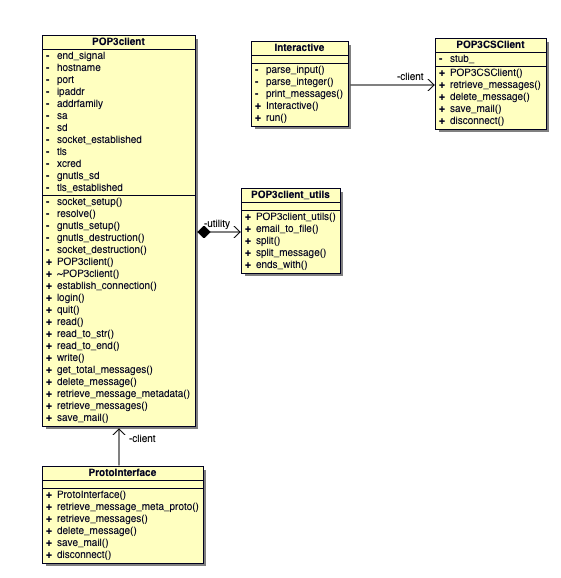
\includegraphics[width=.7\textwidth]{kdg.png}
  \caption{Klassendiagramm}
  \label{fig:kdg}
\end{figure}

\subsection{Klassen}

\subsubsection{POP3client}
Die POP3client Klasse umfasst die Funktionen, die es dem Programm erlauben, eine Verbindung zu einem POP3 Server aufzubauen und dessen Daten auszuwerten.

\subsubsection{POP3client\_utils}
Die POP3client\_utils Klasse umfasst Helfer-Funktionen, die die POP3Client Klasse unterstützen.

\subsubsection{ProtoInterface}
Die ProtoInterface Klasse verarbeitet Daten der POP3Client Klasse und konvertiert diese zu Protobuf Strukturen.

\subsubsection{POP3CSClient}
Die POP3CSClient Klasse ist eine simple gRPC Client Klasse, die Daten des gRPC Servers empfängt und verarbeitet.

\subsubsection{POP3CSImplementation}
Die POP3CSImplementation Klasse umfasst einen simplen gRPC Server.

\subsubsection{Interactive}
Die Interactive Klasse erlaubt die dynamische Eingabe von Befehlen während der Runtime des Programmes. 

\section{Implementierung}
Für Variablen sowie Funktionen wurde "Snake case" benutzt. Sämtliche vorgegebene Codierungskonventionen wurden nach Möglichkeit eingehalten. Um sämtliche Teile des Programmes zu vereinfachen, wurden mehrere externe Bibliotheken verwendet, diese sind in Sektion \ref{extBib} kurz beschrieben. 

\subsection{POP3 Protokoll}
Das Post Office Protocol (POP) ist ein Übertragungsprotokoll, mit dem Clients die Möglichkeit haben, E-Mails von einem E-Mail Server herunterzuladen. Version 3 (POP3) des Protokolls wird im RFC 1939\cite{rfc1939} beschrieben. 

\subsubsection{POP3 Commands}

\paragraph{USER [username]}
Erster Login-Command. Erlaubt es dem Client, einen User anzugeben.

\paragraph{PASS [password]}
Zweiter Login-Command. Erlaubt es dem Client, ein Passwort für den User anzugeben.

\paragraph{STAT}
Gibt die Anzahl von E-Mails und deren totale Größe zurück.

\paragraph{LIST}
Gibt die einzelnen E-Mails und deren Größe zurück.

\paragraph{RETR [message]}
Gibt ein gesammtes E-Mail zurück.

\paragraph{TOP [message]}
Gibt die Metadaten eines E-Mails zurück.

\paragraph{DELE [message]}
Löscht ein E-Mail.

\paragraph{RSET [message]}
Macht das Löschen eines E-Mails rückgängig.

\paragraph{NOOP}
POP3 Server gibt eine Nachricht zurück. Dient nur als Test-Command.

\paragraph{QUIT}
Beendet die Session und speichert getroffene Änderungen.

\section{Kurze Beschreibung diverser Codeblöcke}

\subsection{POP3}

\subsubsection{Auflösen einer Domain}

Die Verwendung der asio Bibliothek war in diesem Projekt leider nicht möglich, daher werden die Domains mit Funktionen aus der netdb.h C Bibliothek aufgelöst.

\begin{code}
\begin{minted}{cpp}
int POP3client::resolve() {
  hostent *rh = gethostbyname(hostname.c_str());
  if(rh == NULL){
      return 1;
  }

  in_addr **ipptr = (struct in_addr**)rh->h_addr_list;

  addrfamily  = rh->h_addrtype;
  ipaddr      = inet_ntoa(*ipptr[0]);
  return 0;
}
\end{minted}
\caption{Auflösen einer Domain ohne asio}
\label{resolve_domain}
\end{code}

\subsubsection{Erstellen einer C Socket}

Da die asio Bibliothek nur TLS über OpenSSL unterstützt, wurde eine normale C Socket implementiert. 

\begin{code}
\begin{minted}{cpp}
int POP3client::socket_setup(){
  int err;

  sd = socket(addrfamily, SOCK_STREAM, 0);
  memset(&sa, '\0', sizeof(sa));

  sa.sin_family = addrfamily;
  sa.sin_port = htons(port);

  inet_pton(addrfamily, ipaddr.c_str(), &sa.sin_addr);
  err = connect(sd, (struct sockaddr *) &sa, sizeof(sa));

  socket_established = true;
  return 0;
}
\end{minted}
\caption{Erstellen einer C Socket}
\label{create_c_socket}
\end{code}

\subsubsection{Implementation von GnuTLS}
\label{gnutls_implement_proj}
Die Funktion aus dem Snippet \ref{create_gnutls} zeigt, wie die Socket aus \ref{create_c_socket} benutzt wird, um einen TLS Handshake zu initialisieren.

\begin{code}
\begin{minted}{cpp}
int POP3client::gnutls_setup(){
  // X.509 authentication is used
  gnutls_global_init();
  gnutls_certificate_allocate_credentials(&xcred);
  gnutls_certificate_set_x509_system_trust(xcred);

  // link socket descriptor to gnutls socket descriptor
  gnutls_transport_set_int(gnutls_sd, sd);

  // initialize handshake
  int err_handshake = gnutls_handshake(gnutls_sd);

  if(err_handshake){
      return 1;
  }

  return 0;
}
\end{minted}
\caption{Gekürzte GnuTLS Setup Funktion}
\label{create_gnutls}
\end{code}

\subsubsection{Lesen aus dem Socket}

Da der Großteil der POP3 Funktionen mit einem Punkt, gefolgt von einem Absatz endet, ist es möglich, größere Nachrichten zu lesen, indem man nach diesem End-Signal sucht.

\begin{code}
\begin{minted}{cpp}
string POP3client::read_to_end(){
  char buff[8000]{};
  memset(buff, 0, sizeof(buff));

  string key = ".\r\n";
  string rec = "";
  string tmp = "";

  while(!utility.ends_with(tmp, key)){
      if(tls){
          gnutls_record_recv(gnutls_sd, buff, sizeof(buff));
      } else {
          recv(sd, buff, sizeof(buff), 0);
      }
      tmp = buff;
      memset(buff, 0, sizeof(buff));

      rec += tmp;
  }
  return rec;
}
\end{minted}
\caption{Funktion, die aus dem Socket liest, bis der Key erreicht wird}
\label{read_to_end}
\end{code}

\subsubsection{Schreiben in das Socket}

Um in das Socket zu schreiben, werden Strings, die den Befehl enthalten, in Char Arrays umgewandelt. Diese werden, basierend darauf ob TLS verwendet wird, mit der dementsprechenden Funktion in das Socket geschrieben.

\begin{code}
\begin{minted}{cpp}
int POP3client::write(std::string msg){
  const char *cmsg = msg.c_str();
  int msg_len = strlen(cmsg);
  int result = 0;
  if(tls){
      result = gnutls_record_send(gnutls_sd, cmsg, msg_len);
  } else {
      result = send(sd, cmsg, msg_len, 0);
  }

  return result;
}
\end{minted}
\caption{Funktion, die in das Socket schreibt}
\label{write_in_socket}
\end{code}

\subsection{Protobuf und gRPC}
\subsubsection{Protobuf}
Protobuf\cite{protobuf} wurde implementiert, um die Verwendung von gRPC für den Austausch von Daten zu ermöglichen.
\begin{code}
  \begin{minted}{c++}
# Message Metadaten
message MailMeta {
  optional int32 message_id = 1;
  optional string from = 2;
  optional string subject = 3;
  optional string date = 4;
}

# Liste von Message Metadaten
message MailList {
  repeated MailMeta mails = 1;
}
  \end{minted}
  \caption{Protobuf Klassen für E-Mail Metadaten sowie eine Liste von diesen}
  \label{proto}
\end{code}

\subsubsection{gRPC}

gRPC\cite{grpc}, auch bekannt als gRPC Remote Procedure Calls, wird benutzt als RPC System. gRPC benutzt HTTP/2 für den Transport und Protocol Buffer als die "interface description language."
% todo erläutern
\begin{code}
  \begin{minted}{c++}
service POP3CS {
  rpc get_mail_list(Operation) returns (MailList) {}

  rpc delete_message(Operation) returns (Success) {}
  rpc save_mail(Operation) returns (Success) {}

  rpc disconnect(Operation) returns (Success) {}
}
  \end{minted}
  \caption{gRPC Routen}
  \label{grpc}
\end{code}

Die POP3CSClient Klasse benutzt einen gRPC Client, um Daten des POP3 Servers über die POP3CSImplementation Klasse anzufragen.

\subsection{Externe Bibliotheken}
\label{extBib}

\subsubsection{CLI11}
CLI11\cite{cli11_ref} ermöglicht eine einfache Verarbeitung von Kommandozeilenargumenten mit eingebauten Methoden zum Überprüfen der angegebenen Werte. Auf diese Argumente wird in Sektion \ref{usage} näher eingegangen.

\subsubsection{tabulate}
Um die E-Mails in einer optisch ansprechenden Art darzustellen, wird eine Tabelle mittels tabulate\cite{tabulate_ref} erstellt.

\begin{code}
  \begin{minted}{text}
bubble> list 3
+------------+----------------------+---------------------------+
| Message ID | Recieved From        | Subject                   | 
+------------+----------------------+---------------------------+
| 6          | David Fischer <...>  | Linkedin ...              | 
+------------+----------------------+---------------------------+
| 5          | David Fischer <...>  | Sie werden wahrgenommen!  |
+------------+----------------------+---------------------------+
| 4          | David Fischer <...>  | DJI MSDK iOS Delay Notice |
+------------+----------------------+---------------------------+
  \end{minted}
  \caption{Ausgabe des $list$ Befehls}
\end{code}

\subsubsection{spdlog}
Um Informationen zu loggen, wird die spdlog\cite{spdlog_ref} Bibliothek verwendet. Die $File Sink$ wird für genauere Details benutzt, während die $Console Sink$ benutzt wird, um die Arbeitsweise des Programms zu demonstrieren.

\begin{code}
\begin{minted}{cpp}
auto console = spdlog::stdout_color_mt("console");
auto logger = spdlog::basic_logger_mt("logger", "logs/basic-log.txt");
\end{minted}
\caption{Erstellen von spdlog Console und File Sinks}
\label{spdlog_code}
\end{code}

\subsubsection{JSON}
Um, wie in Sektion \ref{usage} angemerkt, die Konfiguration aus einem JSON File zu lesen, wird die JSON for modern C++\cite{json_ref} verwendet.

\subsubsection{httplib}
Neben dem $bubble$ executable wird ein executable namens $bubble\_http$ erstellt. Dieses öffnet einen httplib\cite{httplib-ref} HTTP Server auf Port 5001, der es dem Benutzer erlaubt, Mails online mittels gRPC zu verwalten.

\begin{figure}[H]
  \centering
  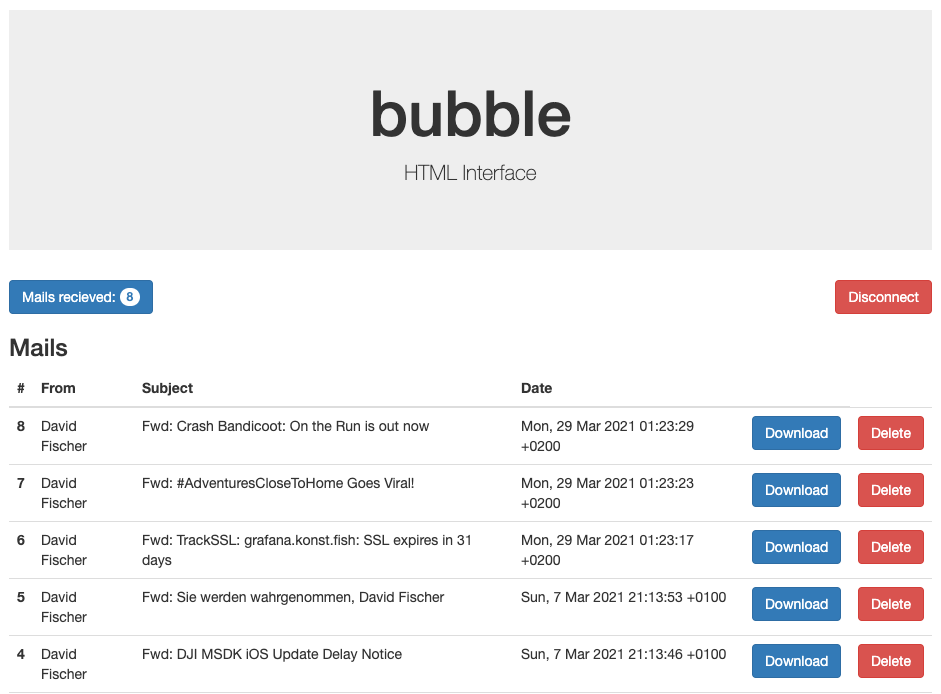
\includegraphics[width=1\textwidth]{web_interface.png}
  \caption{Bubble Web Interface}
  \label{fig:bubble_web_interface}
\end{figure}

\subsubsection{inja}
Um die Web Interface präsentabel darstellen zu können, wird die inja Template Engine\cite{inja-ref} verwendet. In Kombination mit httlib und gRPC kann die Web Interface dynamisch mit Daten befüllt werden.

\subsubsection{GnuTLS}
Um GnuTLS zu implementieren, wurde die C++ API verwendet\cite{gnutls_cpp}. Dies ist in Sektion \ref{gnutls_implement_proj} näher beschrieben.

\section{Verwendung}
\label{usage}

\subsection{Kommandozeilenargumente}

\subsubsection{Konfiguration}
\paragraph{-s,--server}
Domain des POP3 Servers

\paragraph{-u,--user}
Username des Accounts.

\paragraph{-p,--pass}
Username des Accounts.

\paragraph{-t,--tls}
Verbindung mittels TLS etablieren.

\paragraph{--port}
Benutzerdefinierten Port angeben.

\paragraph{-j,--json}
Configuration aus einem JSON File lesen

\subsubsection{Interaktive Eingabe von Befehlen}
\paragraph{-i,--interactive}
Interaktive Eingabe von Befehlen aktivieren.

\begin{code}
  \begin{minted}{text}
bubble> help
Bubble Interactive Client:
dl / download <message_id>  - download email with id
rm / delete <message_id>    - delete email with id
ls / list <amount>          - list amount of mails
exit                        - disconnects the session
help                        - displays this message
  \end{minted}
  \caption{Ausgabe des help Befehls des Interaktiven Clients}
\end{code}

\newpage

\section{Projektstruktur}
\dirtree{%
  .1 /.
  .2 LICENSE.
  .2 meson\_options.txt.
  .2 meson.build.
  .2 README.md.
  .2 RESEARCH.md.
  .2 CHANGELOG.org.
  .2 config.json.
  .2 .gitignore.
  .2 include.
  .3 Interactive.h.
  .3 POP3client.h.
  .3 ProtoInterface.h.
  .3 Util.h.
  .2 src.
  .3 Interactive.cpp.
  .3 main.cpp.
  .3 pop3.proto.
  .3 POP3cilent.cpp.
  .3 ProtoInterface.cpp.
  .3 Util.cpp.
  .2 doc.
  .3 dokumentation.tex.
  .3 references.bib.
  .3 dokumentation.pdf.
  .2 http\_server.
  .3 include.
  .4 POP3CSClient.h.
  .3 src.
  .4 main.cpp.
  .4 POP3CSClient.cpp.
  .2 templates.
  .3 render.html.
  .2 build.
}\hfill

% .bib include & references
\newpage
\bibliography{references}
\bibliographystyle{plain}
\end{document}